\documentclass[12pt, letterpaper]{article}

% ─────────────────────────────────────────────
%  PAQUETES
% ─────────────────────────────────────────────
\usepackage[utf8]{inputenc}
\usepackage[T1]{fontenc}
\usepackage[spanish]{babel}
\usepackage{geometry}
\geometry{
    letterpaper,
    top=2.54cm,
    bottom=2.54cm,
    left=3.0cm,
    right=2.54cm
}

\usepackage{lmodern}
\usepackage{microtype}
\usepackage{graphicx}
\usepackage{float}
\usepackage{setspace}
\setstretch{1.5}
\usepackage{parskip}
\setlength{\parindent}{0pt}
\setlength{\parskip}{6pt}


% Secciones
\usepackage{titlesec}
\titleformat{\section}
    {\normalfont\large\bfseries}
    {\thesection.}{0.8em}{}[\titlerule]
\titleformat{\subsection}
    {\normalfont\normalsize\bfseries}
    {\thesubsection}{0.8em}{}
\titleformat{\subsubsection}
    {\normalfont\normalsize\itshape}
    {\thesubsubsection}{0.8em}{}

% Tablas
\usepackage{booktabs}
\usepackage{tabularx}
\usepackage{array}
\usepackage{longtable}
\usepackage{multirow}

% Matemáticas
\usepackage{amsmath}
\usepackage{amssymb}

% Figuras y captions
\usepackage{caption}
\captionsetup{
    font=small,
    labelfont=bf,
    format=hang,
    margin=1cm
}
\usepackage{tikz}
\usetikzlibrary{shapes.geometric, arrows.meta, positioning}

% Listas
\usepackage{enumitem}

% Hipervínculos
\usepackage[hidelinks]{hyperref}

\usepackage{xcolor}
\definecolor{cBenef}{HTML}{16a34a}    % verde  — beneficio total
\definecolor{cFlujo}{HTML}{2563eb}    % azul   — utilidad / flujo
\definecolor{cCapac}{HTML}{dc2626}    % rojo   — restricción capacidad
\definecolor{cCongest}{HTML}{ea580c}  % naranja — congestión acumulada
\definecolor{cLagrange}{HTML}{7c3aed} % púrpura — coef. Lagrange
\definecolor{cRuta}{HTML}{0891b2}     % cian   — matriz de ruteo

\usepackage{pdflscape}

% Bibliografía desde archivo .bib
\usepackage{csquotes}
\usepackage[
    style=apa,
    backend=biber,
    language=spanish,
    sorting=nyt,
    maxbibnames=99,
    uniquename=init,
    uniquelist=true
]{biblatex}
\DeclareLanguageMapping{spanish}{spanish-apa}
\addbibresource{references.bib}

\begin{document}

\tableofcontents
\newpage

\begin{titlepage}
    \centering

    % Descomenta la siguiente línea y reemplaza el nombre del archivo
    % con el logo de tu institución:
    
\includegraphics[width=5cm]{images/logo_universidad.png}\\[1.0cm]
    \vspace*{1.5cm}


    {\Large\bfseries
        Facultad de Ingenierías\\[0.3em]
        Programa de Ingeniería de Sistemas y Computación
    }

    \vspace{0.8cm}

    {\LARGE\bfseries
        Proyecto Final Comunicaciones II\\[0.3em]
    }


    \vspace{1.0cm}

    {\large
        Integrantes: \\[0.5em]
        Jhoan Esteban Corrales \\[0.2em]
        Juan Camilo Velásquez \\[0.2em]
        Juan Esteban Cardona
    }

    \vfill
    {\normalsize \today}
\end{titlepage}

\section{Introducción}

El presente documento recoge el diseño, la implementación y la validación de
una red empresarial multi-sede que da respuesta a los requerimientos planteados
en el proyecto final de Comunicaciones II como se muestra en la siguiente imagen:

\begin{figure}[H]
      \centering
      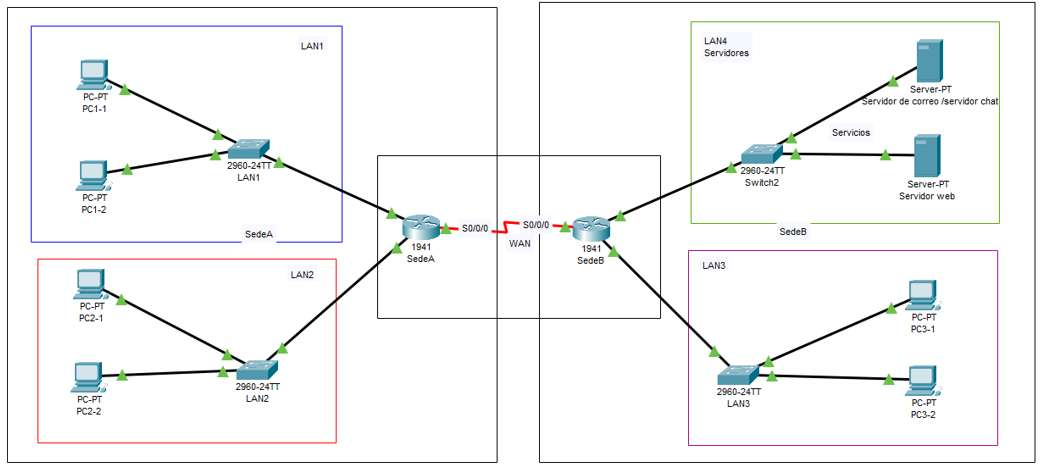
\includegraphics[width=1\textwidth]{images/base.jpg}
      \caption{Diagrama de la red multi-sede a implementar.}
\end{figure}

La red integra tres segmentos LAN con
un total de 1.650 usuarios finales, distribuidos en áreas con capacidades de 850,
600 y 200 hosts respectivamente, y debe garantizar conectividad plena entre todas
las sedes mediante enrutamiento dinámico.

Un requisito del proyecto es la operación en doble stack, de modo que
cada dispositivo de la topología cuente con direccionamiento tanto IPv4 como IPv6.
El espacio de direcciones IPv4 asignado al Grupo 1 es \texttt{172.16.192.0/19},
y el prefijo IPv6 de referencia es \texttt{2001:dbe:bef9::/48}. El diseño del
direccionamiento parte de estos bloques y aplica un factor de crecimiento del 10\%
sobre la cantidad de usuarios de cada área, con el fin de garantizar escalabilidad
sin necesidad de renumerar la red en el corto plazo.

Adicionalmente, la red debe soportar tres servicios de aplicación accesibles desde
todos los segmentos: un servicio web, un servicio de correo electrónico y un
servicio de mensajería instantánea. Este último corresponde a una implementación
propia desarrollada en C sobre sockets TCP, con soporte para múltiples usuarios
simultáneos, salas de chat y visualización de usuarios conectados, operando sobre
terminal tanto en el servidor Linux como en los clientes Windows que se puede ver en el siguiente repositorio: \url{https://github.com/Juanes7222/Socket.git}.

El documento se organiza siguiendo la estructura requerida por el enunciado del
proyecto: inicia con la descripción de requerimientos, continúa con las decisiones
de diseño y la configuración de los equipos, y cierra con el diseño y ejecución de
pruebas de validación, los problemas encontrados durante la implementación y las
conclusiones del proceso.

\section{Descripción de Requerimientos}

\subsection{Requerimientos de Cantidad de Áreas y Redes}

La topología de la empresa comprende tres segmentos LAN independientes,
cada uno asociado a un área funcional de la organización. La cantidad de
usuarios finales por área, antes de aplicar el factor de crecimiento, es
de 850 en LAN 1, 600 en LAN 2 y 200 en LAN 3. Aplicando un crecimiento
previsto del 10\%, las redes deben dimensionarse para albergar 935, 660 y
220 hosts respectivamente, sin contar los dispositivos de telecomunicaciones
ni los servidores de servicios, que requieren subredes dedicadas.

Adicionalmente, la topología contempla una subred de interconexión entre
routers para cada enlace WAN entre sedes, así como una subred dedicada para
los servidores de servicios. En total, el diseño debe prever al menos seis
subredes: tres para usuarios finales, una para servidores, y las necesarias
para los enlaces punto a punto entre dispositivos de enrutamiento.

\subsection{Requerimientos de Direccionamiento}

El espacio de direcciones asignado al Grupo 1 es \texttt{172.16.192.0/19}
para IPv4 y el prefijo \texttt{2001:dbe:bef9::/48} para IPv6. A partir de
estos bloques se debe derivar un esquema de direccionamiento jerárquico que
satisfaga las necesidades de cada segmento de red, considerando los hosts de
usuario final, los dispositivos de telecomunicaciones activos en cada área y
los servidores de servicios.

La estrategia de asignación de direcciones debe definirse de forma diferenciada
según el tipo de dispositivo: servidores, dispositivos de telecomunicaciones y
equipos de usuario final, justificando en cada caso el mecanismo seleccionado
en función de los requerimientos operativos y de administración de la red.

\subsection{Requerimientos de Servicios}

La red debe garantizar la disponibilidad de tres servicios de aplicación
accesibles desde todos los segmentos de la topología a través del enrutador.
El primer servicio es un servidor web que expone contenido HTTP a los usuarios
de todas las áreas. El segundo es un servidor de correo electrónico que permite
el envío y la recepción de mensajes entre los usuarios de la organización. El
tercero es un servicio de mensajería instantánea implementado sobre sockets TCP,
con soporte para salas de chat, visualización de usuarios conectados mediante el
comando \texttt{/list} e historial local de mensajes exportable a archivo de texto.

Los tres servicios se alojan en un servidor Linux con dirección estática dentro
de la subred de servidores, y deben ser accesibles tanto por IPv4 como por IPv6,
en coherencia con el requisito de doble stack definido para toda la topología.

\subsection{Requerimientos de Seguridad}

\subsubsection{Seguridad de Acceso}

Se debe prevenir el acceso no autorizado a los dispositivos de telecomunicaciones
mediante la configuración de credenciales de acceso tanto en la consola local como
en las líneas de terminal virtual. Las contraseñas deben almacenarse de forma
cifrada en los archivos de configuración de los equipos, evitando que queden
expuestas en texto plano dentro de los respaldos de configuración.

En los servidores Linux, el acceso al sistema operativo debe restringirse mediante
reglas de firewall que limiten los puertos expuestos a los estrictamente necesarios
para la operación de cada servicio. Cualquier puerto no requerido por los servicios
web, de correo o de chat debe permanecer cerrado por defecto.

\subsubsection{Seguridad para Configuración Remota}

La administración remota de los dispositivos de telecomunicaciones debe realizarse
exclusivamente a través de SSH versión 2, deshabilitando el protocolo Telnet en
todas las líneas VTY. Esto garantiza que las sesiones de configuración remota
viajen cifradas a través de la red, protegiéndolas frente a ataques de
interceptación pasiva dentro de los mismos segmentos LAN.

Para los servidores Linux, la configuración remota se realizará también mediante
SSH, preferiblemente con autenticación por clave pública en lugar de contraseña,
reduciendo la superficie de ataque frente a intentos de fuerza bruta.

\subsection{Requerimientos de Enrutamiento}

La topología comprende múltiples sedes que deben mantenerse en comunicación
permanente, por lo que se requiere implementar un protocolo de enrutamiento
dinámico que propague automáticamente las rutas hacia todos los segmentos de
la red. El protocolo seleccionado debe operar tanto sobre IPv4 como sobre IPv6,
garantizando conectividad de extremo a extremo para ambas familias de direcciones
en toda la topología.

El diseño del enrutamiento debe contemplar la convergencia de la red ante posibles
cambios en la topología, así como la correcta redistribución de las rutas hacia
las subredes de servidores y enlaces punto a punto, de modo que cualquier
dispositivo final pueda alcanzar cualquier servicio independientemente del área
en la que se encuentre.

\section{Descripción de las Decisiones de Diseño}

\subsection{Esquema de Direccionamiento}

El bloque \texttt{172.16.192.0/19} ofrece 8.190 direcciones utilizables, lo
que permite derivar subredes de tamaño variable mediante VLSM para ajustarse
con precisión a las necesidades de cada segmento. Se optó por este enfoque
en lugar de un esquema de subredes de tamaño fijo, dado que las diferencias
de escala entre las áreas son significativas: LAN 1 requiere más de 900 hosts,
mientras que los enlaces punto a punto entre routers solo necesitan dos
direcciones. Emplear subredes de tamaño uniforme desperdiciaría una fracción
considerable del espacio de direcciones disponible.

Para IPv6, el prefijo \texttt{2001:dbe:bef9::/48} permite asignar subredes
\texttt{/64} a cada segmento de la topología sin restricción práctica de
cantidad. Se adoptó el prefijo \texttt{/64} de forma uniforme para todos los
segmentos, dado que es el tamaño mínimo requerido por SLAAC para la
autoconfiguración de direcciones en los hosts de usuario final, y simplifica
la gestión del plan de direccionamiento al eliminar la necesidad de VLSM en
la familia IPv6.

\subsection{Estrategia de Asignación de Direcciones}

Para los dispositivos de telecomunicaciones y los servidores de servicios se
adoptó asignación de direcciones estática en ambas familias de protocolos.
Esta decisión responde a que dichos dispositivos son puntos críticos de la
infraestructura: una dirección que cambie en un router o en un servidor
invalida rutas configuradas, entradas DNS y reglas de firewall, introduciendo
interrupciones difíciles de diagnosticar en producción. La asignación estática
elimina esta fuente de inestabilidad y facilita la trazabilidad durante la
administración remota.

Para los equipos de usuario final se adoptó asignación dinámica. En IPv4 se
emplea DHCP, de modo que un servidor centralizado distribuye direcciones,
máscara, puerta de enlace y servidor DNS a todos los hosts de cada LAN sin
intervención manual. En IPv6 se emplea SLAAC, mecanismo mediante el cual
cada host construye su propia dirección a partir del prefijo \texttt{/64}
anunciado por el router en sus mensajes Router Advertisement, sin requerir
un servidor dedicado. Esta combinación reduce la carga administrativa en redes
con cientos de usuarios y es coherente con las prácticas estándar en redes
empresariales de escala media.

\subsection{Protocolo de Enrutamiento}

Se seleccionó OSPF como protocolo de enrutamiento dinámico para IPv4, y su
extensión OSPFv3 para IPv6. La elección de OSPF sobre alternativas como RIP
se fundamenta en tres razones principales. Primero, OSPF es un protocolo de
estado de enlace que converge significativamente más rápido que los protocolos
de vector de distancia ante cambios en la topología, lo cual es relevante en
una red multi-sede donde una caída de enlace no debe prolongarse en
inconsistencias de ruteo. Segundo, OSPF no tiene la limitación de 15 saltos
de RIP, lo que lo hace apropiado para topologías que puedan crecer en número
de sedes. Tercero, OSPFv3 extiende de forma nativa el mismo mecanismo a IPv6,
permitiendo mantener una única lógica de enrutamiento para ambas familias de
protocolos.

Toda la topología se configura dentro de una única área OSPF (área 0), dado
que el número de routers no justifica la segmentación en áreas adicionales y
una sola área simplifica la configuración y el diagnóstico.

\subsection{Seguridad en Dispositivos de Telecomunicaciones}

El acceso local a los dispositivos se protege mediante contraseñas cifradas
en consola y en las líneas de terminal virtual. Para la administración remota
se habilita exclusivamente SSHv2, deshabilitando Telnet en todas las líneas
VTY. SSHv2 cifra la sesión completa, incluyendo credenciales y comandos,
lo que impide que un atacante con acceso pasivo a la red pueda capturar
información de configuración sensible.

\subsection{Seguridad en Servidores de Servicios}

En el servidor Linux que aloja los servicios de aplicación se aplica una
política de firewall restrictiva mediante UFW, abriendo únicamente los puertos
correspondientes a cada servicio: 80 para HTTP, 25 y 143 para SMTP e IMAP
respectivamente, y el puerto definido por la implementación del servicio de
chat. El acceso administrativo al sistema operativo se realiza por SSHv2 con
autenticación mediante clave pública, deshabilitando la autenticación por
contraseña en el demonio SSH para reducir la exposición a ataques de fuerza
bruta.

\subsection{Servicios de Aplicación}

El servicio web se implementa sobre Nginx, servidor que ofrece bajo consumo
de recursos y soporte nativo para IPv6 mediante la directiva
\texttt{listen [::]:80}, permitiendo atender conexiones de ambas familias de
protocolos sobre un único proceso. El servicio de correo se implementa con
el stack Postfix y Dovecot: Postfix actúa como agente de transferencia de
correo gestionando los procesos SMTP de envío y recepción, mientras que
Dovecot expone los buzones de usuario mediante IMAP, protocolo que permite
a los clientes acceder al correo sin descargarlo ni eliminarlo del servidor,
lo que es adecuado para un entorno corporativo con múltiples dispositivos
por usuario.

El servicio de mensajería instantánea corresponde a la implementación
desarrollada por el grupo en el reto previo, construida en C sobre sockets
TCP. El servidor opera en Linux y acepta conexiones de clientes Windows a
través de la red. Soporta múltiples usuarios simultáneos, salas de chat
con interacción en canal común, listado de usuarios conectados mediante el
comando \texttt{/list} e historial local de mensajes exportable a archivo
de texto. Para cumplir el requisito de doble stack, el socket del servidor
se configuró con la familia \texttt{AF\_INET6} y la opción
\texttt{IPV6\_V6ONLY} deshabilitada, lo que permite aceptar conexiones tanto
IPv4 como IPv6 sobre un único socket sin modificar la lógica de manejo de
clientes.

\section{Descripción de la Configuración}

\subsection{Configuración del Direccionamiento IPv4}

El plan de direccionamiento IPv4 se construyó a partir del bloque asignado
\texttt{172.16.192.0/19}, aplicando segmentación jerárquica mediante VLSM para
ajustar el tamaño de cada subred a la cantidad real de hosts requeridos en cada
área. Con el crecimiento previsto del 10\% sobre la cantidad de usuarios, LAN 1
requiere capacidad para 936 hosts, LAN 2 para 660 hosts y LAN 3 para 221 hosts.
Por esta razón, LAN 1 y LAN 2 se asignaron con prefijo \texttt{/22}, mientras que
LAN 3 se asignó con prefijo \texttt{/24}, lo que garantiza suficiente espacio
para los equipos finales y permite crecimiento adicional dentro de la misma red.

La red de servidores se asignó en una subred independiente de tamaño reducido,
\texttt{172.16.202.0/29}, con el fin de alojar los servicios centrales de la
infraestructura sin desperdiciar direcciones. De igual forma, los enlaces entre
routers se configuraron con subredes \texttt{/30}, dado que solo requieren dos
direcciones utilizables por enlace. Este criterio reduce el consumo del espacio
de direccionamiento y mantiene una organización clara entre redes de usuarios,
red de servicios y enlaces de interconexión.

La tabla~\ref{tab:ipv4} resume la asignación propuesta para toda la topología.

\begin{table}[H]
\centering
\caption{Plan de direccionamiento IPv4 para el Grupo 1}
\label{tab:ipv4}
\begin{tabularx}{\textwidth}{l l l l l l}
\toprule
Segmento & Red & Prefijo & Primer host & Último host & Broadcast \\
\midrule
LAN 1 & 172.16.192.0 & /22 & 172.16.192.1 & 172.16.195.254 & 172.16.195.255 \\
LAN 2 & 172.16.196.0 & /22 & 172.16.196.1 & 172.16.199.254 & 172.16.199.255 \\
LAN 3 & 172.16.200.0 & /24 & 172.16.200.1 & 172.16.200.254 & 172.16.200.255 \\
Servidores & 172.16.202.0 & /29 & 172.16.202.1 & 172.16.202.6 & 172.16.202.7 \\
Enlace R1-R2 & 172.16.202.8 & /30 & 172.16.202.9 & 172.16.202.10 & 172.16.202.11 \\
\bottomrule
\end{tabularx}
\end{table}

\subsection{Configuración del Direccionamiento IPv6}

Para IPv6 se utilizó el prefijo asignado \texttt{2001:dbe:bef9::/48}, del cual se
derivaron subredes \texttt{/64} para cada segmento de la topología. Esta decisión
permite mantener una estructura uniforme en todos los enlaces y simplifica la
configuración de autoconfiguración en los hosts finales mediante SLAAC. A diferencia
de IPv4, en IPv6 no es necesario ajustar el tamaño de subred según la cantidad de
hosts, por lo que se adoptó una asignación homogénea por segmento.

La tabla~\ref{tab:ipv6} presenta los prefijos utilizados para cada red y la
dirección sugerida para la interfaz del router en cada segmento.

Adicionalmente, la tabla~\ref{tab:servicios} describe los servicios de red implementados en la topología, incluyendo los servidores web y de correo, junto con sus direcciones IP, protocolos utilizados y puertos asociados. Esta información permite identificar claramente los recursos disponibles en la red y los mecanismos de comunicación empleados.

Por otra parte, en la tabla~\ref{tab:hosts} se muestra la asignación de direcciones IPv4 e IPv6 en los hosts finales, donde se evidencia la distribución organizada de direcciones dentro de cada subred, así como la configuración de sus respectivas puertas de enlace para garantizar la conectividad entre redes.

\begin{table}[H]
\centering
\caption{Plan de direccionamiento IPv6 para el Grupo 1}
\label{tab:ipv6}
\begin{tabularx}{\textwidth}{l l l}
\toprule
Segmento & Prefijo IPv6 & Gateway sugerido \\
\midrule
LAN 1 & 2001:dbe:bef9:1::/64 & 2001:dbe:bef9:1::1 \\
LAN 2 & 2001:dbe:bef9:2::/64 & 2001:dbe:bef9:2::1 \\
LAN 3 & 2001:dbe:bef9:3::/64 & 2001:dbe:bef9:3::1 \\
Servidores & 2001:dbe:bef9:10::/64 & 2001:dbe:bef9:10::1 \\
Enlace R1-R2 & 2001:dbe:bef9:ff01::/64 & 2001:dbe:bef9:ff01::1 \\
\bottomrule
\end{tabularx}
\end{table}

\begin{table}[H]
\centering
\caption{Servicios de red y puertos utilizados}
\label{tab:servicios}
\begin{tabularx}{\textwidth}{l l l l l}
\toprule
Servicio & IPv4 & IPv6 (manual) & Puerto & Tipo \\
\midrule
Servidor Web & 172.16.202.6 & 2001:dbe:bef9:10::10 & 80 & HTTP \\
Servidor Correo (SMTP) & 172.16.202.5 & 2001:dbe:bef9:10::11 & 25 & SMTP \\
Servidor Correo (POP3) & 172.16.202.5 & 2001:dbe:bef9:10::11 & 110 & POP3 \\
\bottomrule
\end{tabularx}
\end{table}

\begin{table}[H]
\centering
\caption{Asignación de direcciones IP en hosts}
\label{tab:hosts}
\begin{tabularx}{\textwidth}{l l l l l}
\toprule
Dispositivo & Red & IPv4 & IPv6 (manual) & Gateway \\
\midrule
PC1-1 & LAN 1 & 172.16.192.253 & 2001:dbe:bef9:1::10 & 172.16.192.1 \\
PC1-2 & LAN 1 & 172.16.192.254 & 2001:dbe:bef9:1::11 & 172.16.192.1 \\
PC2-1 & LAN 2 & 172.16.196.253 & 2001:dbe:bef9:2::10 & 172.16.196.1 \\
PC2-2 & LAN 2 & 172.16.196.254 & 2001:dbe:bef9:2::11 & 172.16.196.1 \\
PC3-1 & LAN 3 & 172.16.200.253 & 2001:dbe:bef9:3::10 & 172.16.200.1 \\
PC3-2 & LAN 3 & 172.16.200.254 & 2001:dbe:bef9:3::11 & 172.16.200.1 \\
\bottomrule
\end{tabularx}
\end{table}

\subsection{Configuración de los Equipos de Red}

Los routers de la topología se configuran con direccionamiento estático en
ambas familias de protocolos. Cada interfaz conectada a una LAN recibe una
dirección de puerta de enlace dentro del rango correspondiente, mientras que
las interfaces de interconexión entre routers utilizan las subredes punto a
punto definidas anteriormente. Esta organización facilita la administración de
rutas y permite identificar con claridad el papel de cada interfaz dentro de la
topología.

En los dispositivos de acceso y conmutación se habilitan contraseñas locales y
acceso remoto seguro mediante SSHv2. El protocolo Telnet no se utiliza, debido
a que transmite credenciales sin cifrado. Adicionalmente, se limita el acceso
administrativo únicamente a las direcciones internas de la red, de forma que
la configuración remota solo pueda realizarse desde los segmentos autorizados.

\subsection{Configuración de los Servidores y Despliegue Físico}

Aunque el diseño lógico prevé un gran clúster de servidores para atender la demanda total teórica, el despliegue práctico para la validación de esta topología se realiza mediante un esquema distribuido de dos máquinas virtuales (VMs) corriendo Ubuntu 26.04 . Cada máquina virtual fue aprovisionada con 3 núcleos de procesamiento (vCPUs) y 8 GB de memoria RAM, garantizando recursos suficientes para la operación fluida de los servicios en un entorno representativo.

Ambos servidores cuentan con direcciones IP fijas dentro de la subred \texttt{172.16.202.0/29} (con equivalentes IPv6 en \texttt{2001:dbe:bef9:10::/64}):
\begin{itemize}
    \item \textbf{VM 1 (Servidor Web y Portal):} Aloja el portal React/Vite servido mediante Nginx, así como el \textit{backend} en Python (FastAPI) que provee la API REST y los WebSockets.
    \item \textbf{VM 2 (Servidor de Correo y Chat):} Dedicada a los servicios persistentes en segundo plano, corriendo el sistema de mensajería desarrollado en C, además de los demonios Postfix y Dovecot para el correo corporativo.
\end{itemize}

La asignación fija es necesaria para asegurar que los clientes de todas las LAN puedan localizar los servicios de forma consistente en los registros DNS sin depender de mecanismos dinámicos.

El aseguramiento (\textit{hardening}) del SO en estos servidores se orquesta de manera automatizada mediante nuestros scripts de despliegue. En lugar de configuraciones iterativas y manuales, los parámetros de red, el endurecimiento de SSHv2, las contramedidas perimetrales usando UFW y los permisos granulares para la creación de usuarios o encendido de demonios, son inyectados mediante los ejecutables durante la etapa de provisión. La descripción completa de estas políticas de seguridad estructurales se profundiza en las decisiones de diseño.

\subsection{Configuración de los Clientes}

Los equipos de usuario final reciben su configuración de red de manera dinámica.
En IPv4 se emplea DHCP para distribuir dirección IP, máscara, puerta de enlace
y servidor DNS. En IPv6 se utiliza SLAAC, de modo que los clientes generan su
propia dirección a partir del prefijo anunciado por el router en cada segmento.
Esta estrategia disminuye la carga administrativa y facilita la puesta en marcha
de un número elevado de clientes en laboratorio.

El cliente de mensajería instantánea desarrollado en Windows se conecta al
servidor Linux mediante la dirección asignada en la red de servicios, y utiliza
la interfaz de terminal para interactuar con el sistema. El soporte de historial
local, listado de usuarios conectados y salas de chat se valida directamente
sobre la conectividad establecida entre los segmentos de la red.



\begin{landscape}

\section{Diseño Lógico de la Topología}

\begin{figure}[H]
\centering
\begin{tikzpicture}[
    font=\small,
    % Cambiamos los routers a forma circular (estándar)
    router/.style={draw, circle, thick, minimum size=1.8cm, align=center, fill=blue!10},
    switch/.style={draw, rounded corners, thick, minimum width=2.7cm, minimum height=0.9cm, align=center, fill=gray!15},
    server/.style={draw, rounded corners, thick, minimum width=2.8cm, minimum height=0.9cm, align=center, fill=green!15},
    client/.style={draw, rounded corners, thick, minimum width=2.5cm, minimum height=0.8cm, align=center, fill=orange!15},
    % Las conexiones de red no llevan flechas direccionales
    link/.style={thick, draw=black!80},
    % Estilos para etiquetas de interfaces y subredes
    intf/.style={font=\scriptsize, text=black!70},
    subnet/.style={font=\scriptsize\bfseries, text=black}
]

% --- Fondos para agrupar las sedes ---
\draw[dashed, draw=gray!80, fill=gray!5, rounded corners=15pt] (-6.5, 1.5) rectangle (5.5, -5.5);
\node[font=\large\bfseries, text=gray] at (-4, 1) {SEDE A};

\draw[dashed, draw=gray!80, fill=gray!5, rounded corners=15pt] (5.8, 1.5) rectangle (16.5, -5.5);
\node[font=\large\bfseries, text=gray] at (14, 1) {SEDE B};

% --- Routers ---
\node[router] (r1) at (0,0) {Router 1\\Sede A};
\node[router] (r2) at (11,0) {Router 2\\Sede B};

% --- Enlace WAN ---
\draw[link] (r1) -- node[above, subnet] {172.16.202.8/30} node[pos=0.15, intf, above] {S0/0/0} node[pos=0.85, intf, above] {S0/0/0} (r2);

% --- SEDE A - LAN 1 ---
\node[switch] (sw1) at (-3,-2.5) {SW-LAN1};
\node[client] (c1a) at (-4.5,-4) {Host 1-1};
\node[client] (c1b) at (-1.5,-4) {Host 1-2};

\draw[link] (r1) -- node[pos=0.2, intf, left=2pt] {G0/0} node[pos=0.7, subnet, left=4pt, align=right] {LAN 1\\172.16.192.0/22} (sw1);
\draw[link] (sw1) -- (c1a);
\draw[link] (sw1) -- (c1b);

% --- SEDE A - LAN 2 ---
\node[switch] (sw2) at (3,-2.5) {SW-LAN2}; 
\node[client] (c2a) at (1.3,-4) {Host 2-1};
\node[client] (c2b) at (4,-4) {Host 2-2};

\draw[link] (r1) -- node[pos=0.2, intf, right=2pt] {G0/1} node[pos=0.7, subnet, right=4pt, align=left] {LAN 2\\172.16.196.0/22} (sw2);
\draw[link] (sw2) -- (c2a);
\draw[link] (sw2) -- (c2b);

% --- SEDE B - LAN 3 ---
\node[switch] (sw3) at (8,-2.5) {SW-LAN3};
\node[client] (c3a) at (7,-4) {Host 3-1};
\node[client] (c3b) at (9.5,-4) {Host 3-2};

\draw[link] (r2) -- node[pos=0.2, intf, left=2pt] {G0/0} node[pos=0.7, subnet, left=4pt, align=right] {LAN 3\\172.16.200.0/24} (sw3);
\draw[link] (sw3) -- (c3a);
\draw[link] (sw3) -- (c3b);

% --- SEDE B - LAN 4 ---
\node[switch] (sw4) at (13.5,-2.5) {SW-Servidores};
\node[server] (srv1) at (12,-4) {Servidor\\Web};
\node[server] (srv2) at (15,-4) {Servidor\\Correo/Chat};

\draw[link] (r2) -- node[pos=0.2, intf, right=2pt] {G0/1} node[pos=0.7, subnet, right=4pt, align=left] {LAN 4 (Servicios)\\172.16.202.0/29} (sw4);
\draw[link] (sw4) -- (srv1);
\draw[link] (sw4) -- (srv2);

\end{tikzpicture}
\caption{Topología lógica con asignación de interfaces y subredes IPv4}
\label{fig:topologia}
\end{figure}

\end{landscape}

\end{document}
